\chapter{DESAIN DAN IMPLEMENTASI}
\label{chap:desainimplementasi}

\section{Metode yang dirancang}
\label{sec:metode yang dirancang}

Metode yang dirancang pada penelitian ini sebagaimana ditunjukkan pada Gambar \ref{fig:metode}

\begin{figure}[H]
  \centering
  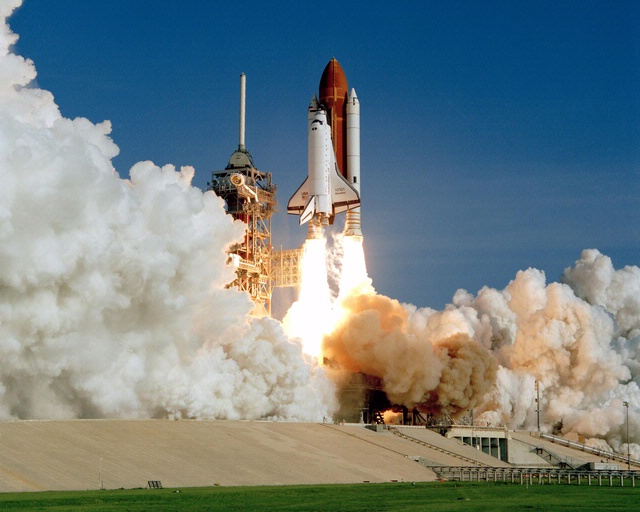
\includegraphics[scale=0.35]{gambar/roketluarangkasa.jpg}

  % Ubah dengan keterangan gambar yang diinginkan
  \caption{Diagram Alir Metode Penelitian}
  \label{fig:metode}
\end{figure}
% what else except nolistsep?

\begin{itemize}[topsep=0pt]
  \item \textbf{Studi Literatur}
  
  Pada tahap ini dilakukan riset studi literatur mengenai konsep dan permasalahan-permasalahan yang sudah ada terkait DISC, Apache Spark, Titian, DistilGPT2, dan FastAPI. Studi literatur didapatkan melalui buku, internet, jurnal penelitian, dan materi-materi kuliah yang berkaitan dengan metode yang akan digunakan.

  \item \textbf{Perancangan Arsitektur Sistem}
  
  \begin{figure}[H]
    \centering
    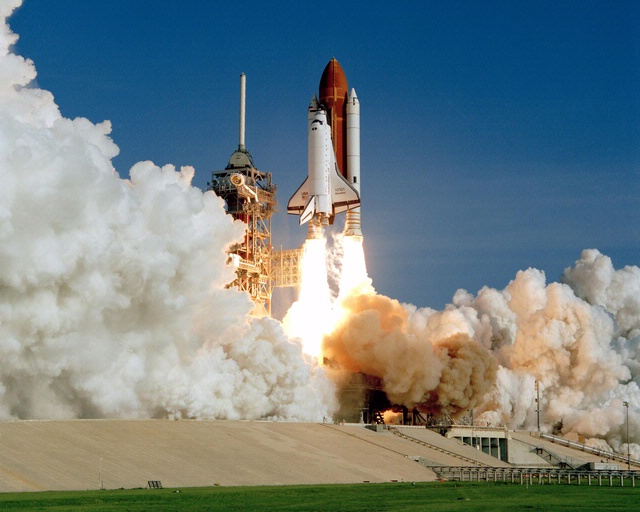
\includegraphics[scale=0.35]{gambar/roketluarangkasa.jpg}
  
    % Ubah dengan keterangan gambar yang diinginkan
    \caption{Rancangan Arsitektur Sistem}
    \label{fig:arsitektur}
  \end{figure}
  
  Tahap perancangan arsitektur sistem dilakukan dengan mengombinasikan dasar teori pada bab 2. Perancangan metode akan dimulai dari proses pemisahan dataset berdasarkan data yang benar dan yang bermasalah, generate input beserta re-training, pengaksesan model menggunakan FastAPI yang di-deploy di AWS EC2, hingga penggabungan keseluruhan proses menjadi satu arsitektur utuh yang dapat di lihat pada Gambar \ref{fig:arsitektur}.

  \item \textbf{Perancangan Metode Generate Input}
  
  \begin{figure}[H]
    \centering
    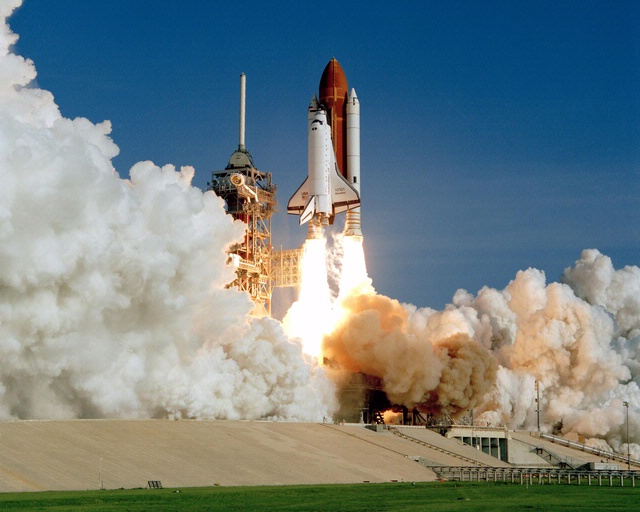
\includegraphics[scale=0.35]{gambar/roketluarangkasa.jpg}
  
    % Ubah dengan keterangan gambar yang diinginkan
    \caption{Rancangan Metode Generate Input}
    \label{fig:generateinput}

  \end{figure}
  
  Tahap perancangan metode generate input dilakukan dengan melakukan proses traning dan re-training terhadap DistilGPT2 model. Tahap ini dapat ditunjukkan melalui Gambar \ref{fig:generateinput}.

  \item \textbf{Pengembangan Sistem}
  
  Pengembangan sistem dilakukan dengan menerapkan algoritma solusi yang dirancang pada subbab perancangan arsitektur sistem dan perancangan metode generate input. Untuk API yang dihasilkan pada perancangan metode generate input akan menggunakan bahasa pemrograman python, sedangkan untuk sistem secara keseluruhan akan menggunakan bahasa pemrograman Scala. Kode program penelitian ini dirancang untuk dapat dipasangkan ke sebuah program yang merupakan program target dilakukannya proses debugging dan generate test input di sistem DISC Apache Spark. Pada saat program target tersebut dijalankan, program pada penelitian ini akan memonitor data input, melakukan re-training model terhadap data yang benar, dan akan melakukan proses generate test input baru untuk menggantikan test input yang bermasalah. 

  \item \textbf{Analisis Kinerja Sistem}
  
  Analisis kinerja sistem yang akan dilakukan pada penelitian ini ada dua, yaitu yaitu pada proses pemisahan dataset dan pada proses generate dataset baru. Analisis kinerja sistem pada proses pemisahan dataset dilakukan dengan menghitung nilai accuracy pada sejumlah program yang akan ditargetkan di mana masing-masing datasetnya akan dilabeli dari awal antara data yang benar dan data yang bermasalah. Untuk analasis kinerja sistem pada proses generate dataset baru dilakukan dengan menghitung persentase dataset benar yang berhasil digenarate oleh model ditiap iterasinya. Proses penentuan apakah dataset baru benar atau bermasalah akan dilakukan secara manual dengan melihat dataset yang telah ada.

  \item \textbf{Penyusunan Laporan Tugas Akhir}
  
  Tahap ini merupakan tahap akhir dari penelitian ini yaitu penyusunan laporan dalam bentuk buku tugas akhir yang menjelaskan dasar teori dan metode yang digunakan dalam tugas akhir ini serta hasil implementasi yang telah dibuat. Sistematika penulisan buku tugas akhir secara garis besar antara lain:

  \begin{enumerate}[topsep=0pt]
    \item Pendahuluan
    \begin{enumerate}[topsep=0pt]
      \item Latar Belakang
      \item Rumusan Masalah
      \item Batasan Tugas Akhir
      \item Tujuan
      \item Metodologi
    \end{enumerate}
    \item Tinjauan Pustaka
    \item Desain dan Implementasi
    \item Pengujian dan Evaluasi
    \item Kesimpulan dan Saran
    \item Daftar Pustaka
  \end{enumerate}
\end{itemize}

\section{Peralatan Pendukung}
\label{sec:peralatan pendukung}

Terdapat beberapa peralatan hardware dan software pendukung yang digunakan untuk pengembangan sistem pada Tugas Akhir ini yang dapat dilihat sebagai berikut:
\begin{itemize}[topsep=0pt]
  \item Hardware
  \begin{enumerate}[topsep=0pt]
    \item Laptop MacBook Pro M2
  \end{enumerate}
  \item Software
  \begin{enumerate}[topsep=0pt]
    \item Google Colaboratory
    \item Visual Studio Code
    \item IntelliJ IDEA CE
    \item HuggingFace
    \item Amazon Web Service EC2
  \end{enumerate}
\end{itemize}
\section{Implementasi}
\label{sec:implementasi}
Tujuan utama dari penelitian ini adalah menghasilkan data 
yang menyebabkan kesalahan dalam jumlah yang dapat dengan 
mudah dianalisis oleh developer. 
Gambar \ref{fig:alur kerja teknik} merangkum alur 
kerja teknik kami. Teknik ini dimulai 
dengan penyesuaian awal arsitektur \emph{generative LLM} yang 
sudah dilatih sebelumnya menggunakan sampel acak dari data. 
LLM ini di-host di server langsung dan diakses melalui API 
khusus yang dijelaskan di Tabel \ref{tab:api}. Ketika ditemukan eksekusi 
program yang salah, penelitian kami menggunakan Titain, sebuah 
\emph{provenance engine}, untuk mendapatkan serangkaian baris yang 
mencurigakan. Sampel data yang dilatih ini memiliki 
persentase lebih tinggi dari baris yang menyebabkan kesalahan, 
yang kemudian digunakan untuk lebih menyesuaikan generative 
LLM, sehingga model ini mempelajari pola dasar dari input yang 
menyebabkan kesalahan dan cenderung menghasilkan baris 
yang salah. Akhirnya, dengan menggunakan model ini, 
kami mendorongnya untuk menghasilkan 
sampel baris, secara bertahap meningkatkan jumlah baris 
yang dihasilkan hingga \emph{bug} tersebut terdeteksi kembali.
Dalam membuat Tugas Akhir ini, terdapat beberapa proses 
yang perlu dilakukan sesuai pada gambar \ref{fig:diagram alir implementasi}

\begin{figure}[H]
  \centering
  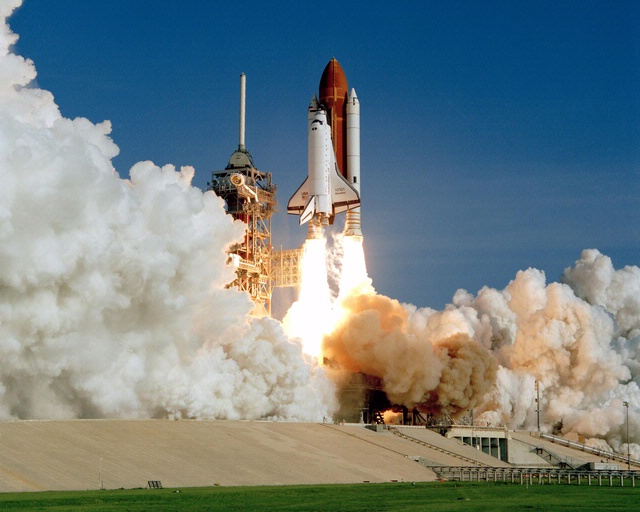
\includegraphics[scale=0.35]{gambar/roketluarangkasa.jpg}

  % Ubah dengan keterangan gambar yang diinginkan
  \caption{Alur Kerja Teknik}
  \label{fig:alur kerja teknik}
\end{figure}

\begin{table}[H]
  \centering
  \caption{Tabel API}
  \begin{tabular}{|c|c|}
    \hline
    \textbf{API} & \textbf{Deskripsi} \\
    \hline
    \texttt{GET /generate} & Menghasilkan input yang menyebabkan kesalahan \\
    \hline
    \texttt{POST /retrain} & Melatih model dengan data yang benar \\
    \hline
  \end{tabular}
  \label{tab:api}
\end{table}

\begin{figure}[H]
  \centering
  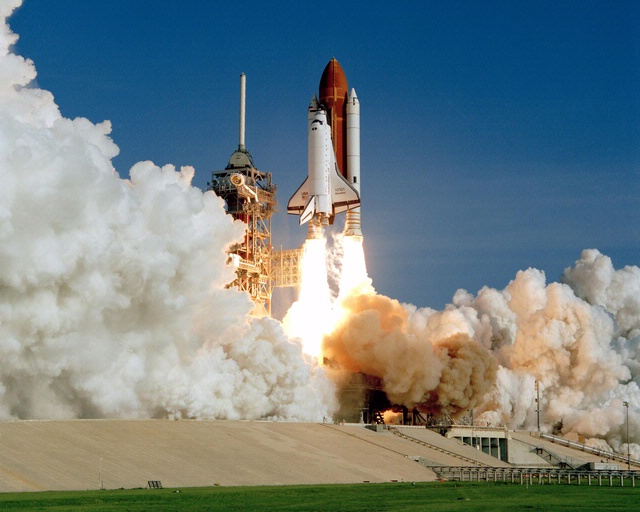
\includegraphics[scale=0.35]{gambar/roketluarangkasa.jpg}

  % Ubah dengan keterangan gambar yang diinginkan
  \caption{Diagram Alir Rencana Implementasi dan Uji Coba}
  \label{fig:diagram alir implementasi}
\end{figure}

\subsection{Mengambil Input yang Menimbulkan Kesalahan dari Eksekusi yang Salah}
\label{sec:mengambil input}

Alat kami pertama-tama menggunakan \emph{provenance tool} 
seperti Titian untuk mendapatkan sampel input yang bias 
terhadap baris-baris yang menginduksi kesalahan dalam eksekusi 
program tertentu. Ketika analis data mengeksekusi program 
dengan data asli, alat kami menggunakan \emph{API call} 
{\tt LLM\_pretrain(orig\_data\_path)} untuk memberikan data 
awal ke server \emph{LLM}. Tujuan dari data ini adalah untuk 
membiasakan \emph{LLM} dengan format dan skema data. 
Perlu dicatat bahwa karena \emph{LLM} menggunakan 
\emph{pre-trained weights} dari GPT-2, tidak diperlukan 
sejumlah besar data untuk dapat menghasilkan baris dengan 
format yang diharapkan. Akibatnya, waktu pelatihan untuk 
langkah ini relatif singkat.

Ketika eksekusi program menghasilkan keluaran yang 
mencurigakan, analis dapat menentukan aturan filter 
menggunakan \emph{Titian's API} untuk mengidentifikasi 
kemungkinan penyebab keluaran yang salah. Data penyebab 
yang dikembalikan oleh Titian bisa sangat besar sehingga 
tidak mungkin dianalisis oleh pengembang manusia, misalnya, 
hingga jutaan baris. Wawasan kami adalah bahwa meskipun data 
penyebabnya besar, inti dari kesalahan dapat ditangkap dalam 
beberapa baris saja. Model bahasa modern adalah alat yang 
berguna untuk menangkap pola-pola yang menginduksi kesalahan 
dari sampel bias yang dikembalikan oleh Titian.

\subsection{Melatih Model Bahasa Pembangkitan Input yang Menginduksi Kesalahan Secara Offline}
\label{sec:melatih model}

Setelah sekumpulan baris potensial yang menyebabkan keluaran 
yang salah diperoleh, alat kami menggunakan \emph{API call} 
{\tt LLM\_pretrain(faulty\_sample)} untuk melatih ulang model 
dengan data yang dicurigai dan membiasakannya untuk 
menghasilkan input yang menginduksi kesalahan. \emph{LLM} 
mengambil baris-baris ini dan menerapkan proses pelatihan 
awal sekali lagi menggunakan baris-baris yang salah yang 
disediakan.

\subsection{Pembuatan Input yang Menginduksi Kesalahan secara Ringkas}
\label{sec:pembuatan input}

Dengan menggunakan model yang bias, alat kami dapat 
menghasilkan input baru yang menginduksi kesalahan untuk 
mereproduksi gejala kesalahan yang sama dengan data yang 
jauh lebih sedikit. Karena model yang dilatih adalah 
\emph{generative LLM}, kami dapat menggunakan 
\emph{API call} {\tt LLM\_generate(N)} untuk menghasilkan 
N baris data. Idealnya, N yang dibutuhkan untuk mereproduksi 
kesalahan harus cukup kecil agar mudah dianalisis oleh 
programmer manusia. Secara analitis, menentukan nilai N 
sangat sulit, jika tidak bisa dibilang mustahil. Oleh 
karena itu, alat kami mengambil pendekatan iteratif. 
Alat ini memulai dengan memanggil {\tt LLM\_generate(1)} 
dan mengeksekusi program menggunakan baris yang dihasilkan. 
Jika gejala kesalahan terproduksi, loop berhenti. Jika tidak, 
alat ini meningkatkan N secara logaritmik hingga kesalahan 
terproduksi. Jika alat ini tidak dapat mereproduksi kesalahan 
dalam jumlah iterasi yang ditentukan oleh pengguna, loop akan 
dihentikan dan alat melaporkan kegagalan untuk mereproduksi 
kesalahan.

\subsection{Mengunggah API ke Layanan Cloud}
\label{sec:mengunggah api}

Setelah model telah berhasil dilatih untuk menghasilkan 
input yang menginduksi kesalahan dan diuji untuk memastikan 
efektivitasnya, langkah selanjutnya adalah mengunggah 
\emph{API} ke layanan \emph{cloud}. Mengunggah \emph{API} 
ke layanan \emph{cloud} memungkinkan akses yang mudah dan 
skalabilitas untuk pengguna di berbagai lokasi. Dengan 
menggunakan \emph{API} yang diunggah ke \emph{cloud}, 
pengembang dapat mengotomatisasi proses deteksi dan 
reproduksi kesalahan tanpa perlu mengelola infrastruktur 
secara langsung. Layanan \emph{cloud} juga menyediakan 
sumber daya yang diperlukan untuk menangani permintaan 
\emph{API} dalam jumlah besar, memastikan bahwa alat 
tetap responsif dan efisien bahkan di bawah beban kerja 
yang tinggi. Langkah ini melibatkan konfigurasi server 
\emph{cloud} untuk menjalankan \emph{LLM} dan mengatur 
\emph{endpoint API} untuk menerima dan memproses permintaan 
dari pengguna, memungkinkan integrasi yang mulus dengan 
berbagai sistem dan aplikasi.

% Contoh pembuatan potongan kode
\begin{lstlisting}[
  language=C++,
  caption={Program halo dunia.},
  label={lst:halodunia}
]
#include <iostream>

int main() {
    std::cout << "Halo Dunia!";
    return 0;
}
\end{lstlisting}

\lipsum[2-3]

% Contoh input potongan kode dari file
\lstinputlisting[
  language=Python,
  caption={Program perhitungan bilangan prima.},
  label={lst:bilanganprima}
]{program/bilangan-prima.py}


\lstinputlisting[
  caption={Program perhitungan bilangan prima.},
  label={lst:contoh-pseudocode}
]{program/contoh-pseudocode.txt}
